\section{K. 데이터 제작}

\begin{frame} % No title at first slide
    \sectiontitle{K}{데이터 제작}
    \sectionmeta{
        \texttt{constructive}\\
        출제진 의도 -- \textbf{\color{acdiamond}Hard}
    }
    \begin{itemize}
        \item 제출 36번, 정답 5팀 (정답률 13.89\%)
        \item 처음 푼 팀: \textbf{여기가월파2020인가요} (월파, 치러, 왔어요), 171분
        \item 출제자: \texttt{jhnah917}
    \end{itemize}
\end{frame}

\begin{frame}{\textbf{K}. 데이터 제작}
    문제 만들어서 Call for Tasks 제출할 때까지만 해도 \difficulty{15}정도 예상했는데, 검수진분들이 \difficulty{21}을 주셨습니다. (???)
\end{frame}

\begin{frame}{\textbf{K}. 데이터 제작}
    문제를 간단하게 요약해봅시다.
    
    \vspace{18pt}
    
    \begin{itemize}
        \item 정점이 $N$개, 간선이 $M$개, 면이 $K$개인 평면 그래프를 만들자. (outer face 제외)
        \item self loop와 multi edge가 없어야 한다.
        \item \textbf{(중요) 좌표 범위 제한이 있다.}
    \end{itemize}
    
    \vspace{18pt}
    
    좌표 범위 제한만 없으면 아주 쉬운 문제인데, 좌표 제한 때문에 어려운 문제가 되었습니다.
\end{frame}

\begin{frame}{\textbf{K}. 데이터 제작}
    평면 그래프의 $V, \space E, \space F, \space C$를 각각 정점, 간선, 면, 컴포넌트의 개수라고 하면, $V-E+F=C+1$이 성립합니다.

    
    $N = V, \space M = E, \space K = F-1$이므로 $N-M+K=C$입니다.
    
    \vspace{18pt}
    
    self loop와 multi edge가 없는 평면 그래프에서는 $M \leq 3N-6$이 성립합니다.
    
    그러므로 $N$개의 정점과 $3N-6$개의 간선을 좁은 공간 안에 다 밀어넣는 방법을 찾은 뒤, $M < 3N-6$이라면 간선을 적당히 제거해주면 됩니다.
    
    \vspace{18pt}
    
    $C \neq 1$인 경우에는 정점 $C-1$개를 따로 빼내면 $C = 1$인 상황으로 만들 수 있습니다.
\end{frame}

\begin{frame}{\textbf{K}. 데이터 제작}
    좌표 범위를 신경쓰지 않고, $3N-6$개의 간선을 만드는 방법을 알아봅시다.
\end{frame}

\begin{frame}{\textbf{K}. 데이터 제작}
    \begin{figure}[h!]
        \centering
        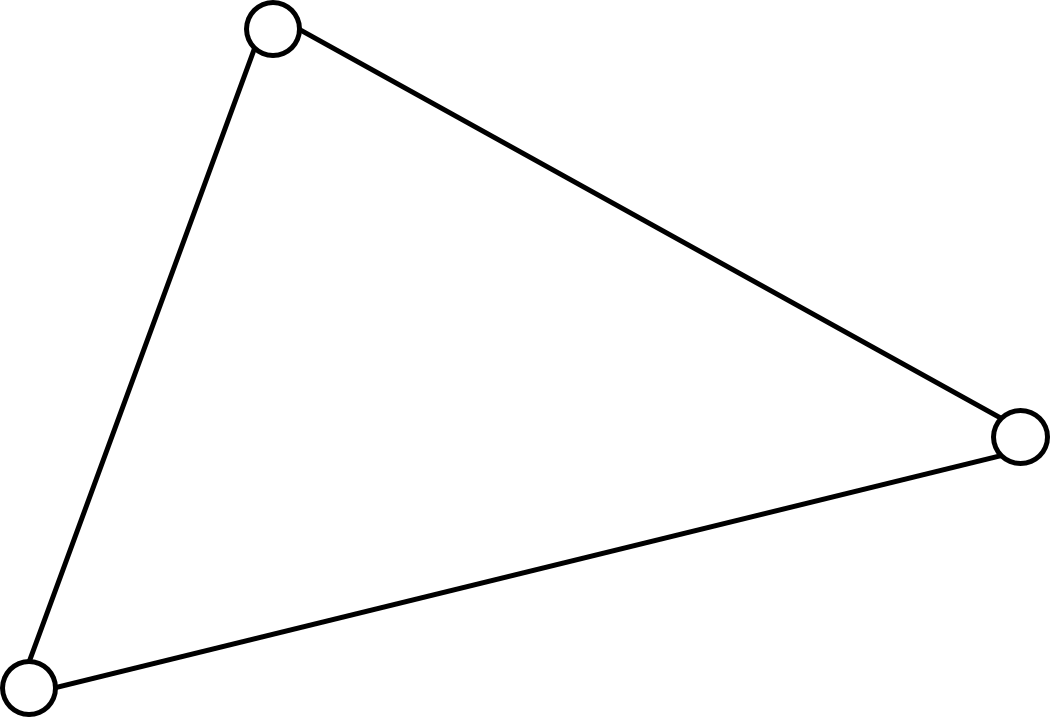
\includegraphics[width=0.35\linewidth]{../images/v-e-f/sol1.png}
    \end{figure}
    
    충분히 큰 삼각형에서 시작합니다.
    
    정점은 $3$개, 간선은 $3(=3\times3-6)$개 있습니다.
\end{frame}

\begin{frame}{\textbf{K}. 데이터 제작}
    \begin{figure}[h!]
        \centering
        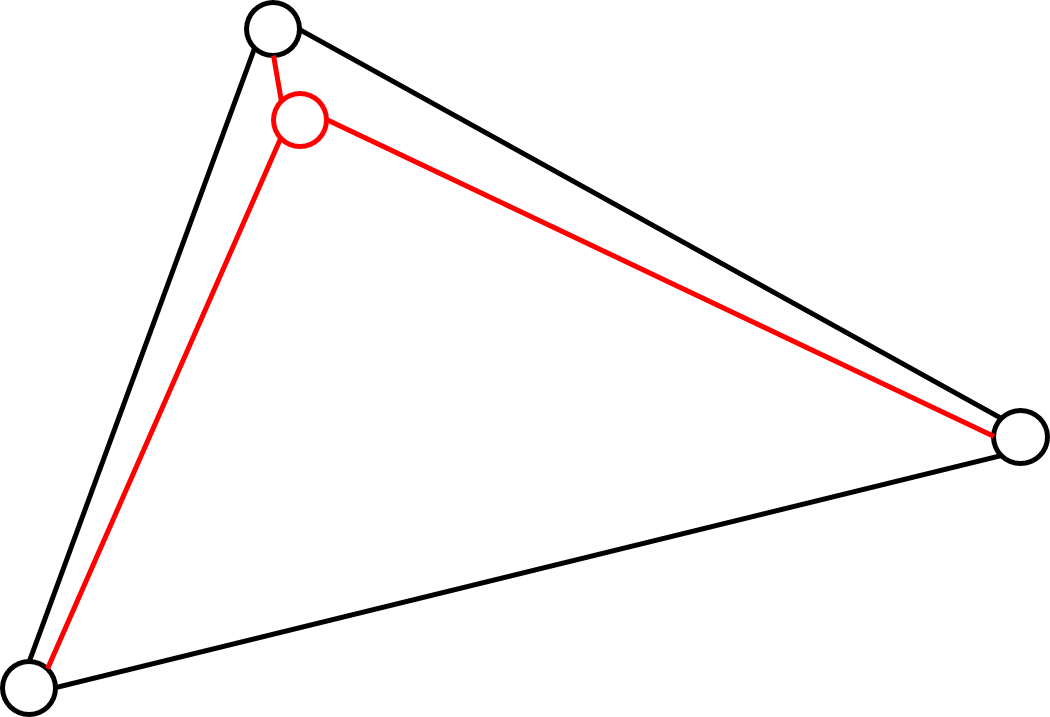
\includegraphics[width=0.35\linewidth]{../images/v-e-f/sol2.png}
    \end{figure}
    
    전 단계에서 만든 삼각형 내부에 점 하나를 찍으면
    
    정점 $1$개와 간선 $3$개를 만들 수 있습니다.
\end{frame}

\begin{frame}{\textbf{K}. 데이터 제작}
    \begin{figure}[h!]
        \centering
        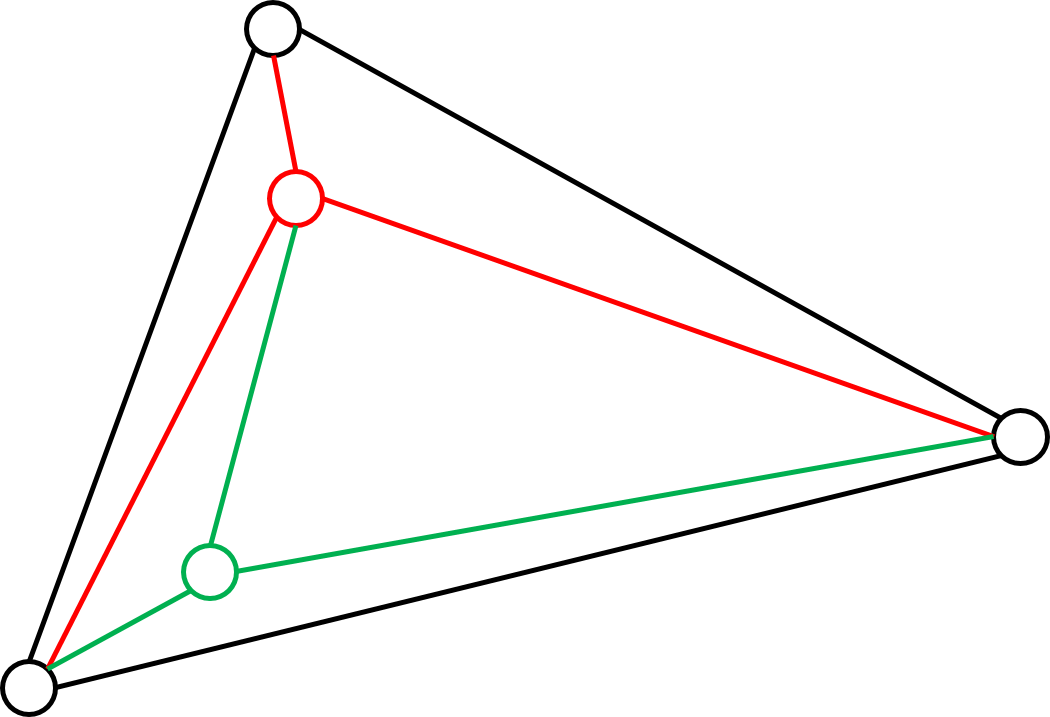
\includegraphics[width=0.35\linewidth]{../images/v-e-f/sol3.png}
    \end{figure}
    
    점 하나를 추가해서 만들어진 삼각형 내부에 점을 추가하면
    
    정점 $1$개와 간선 $3$개를 또 만들 수 있습니다.
    
    \vspace{18pt}
    
    점이 $N$개 생길 때까지 반복하면 됩니다.
\end{frame}

\begin{frame}{\textbf{K}. 데이터 제작}
    모든 영역을 삼각형으로 만들어주면 간선이 $3N-6$개가 된다는 것을 알았습니다.
    
    \vspace{18pt}
    
    이제 최대한 좁은 공간에 넣어봅시다.
    
    정점 3개로 큰 삼각형을 만들고\\
    그 안에 나머지 $N-3$개의 점을 넣을 수 있어야 합니다.
\end{frame}

\begin{frame}{\textbf{K}. 데이터 제작}
    
    \begin{figure}[h!]
        \centering
        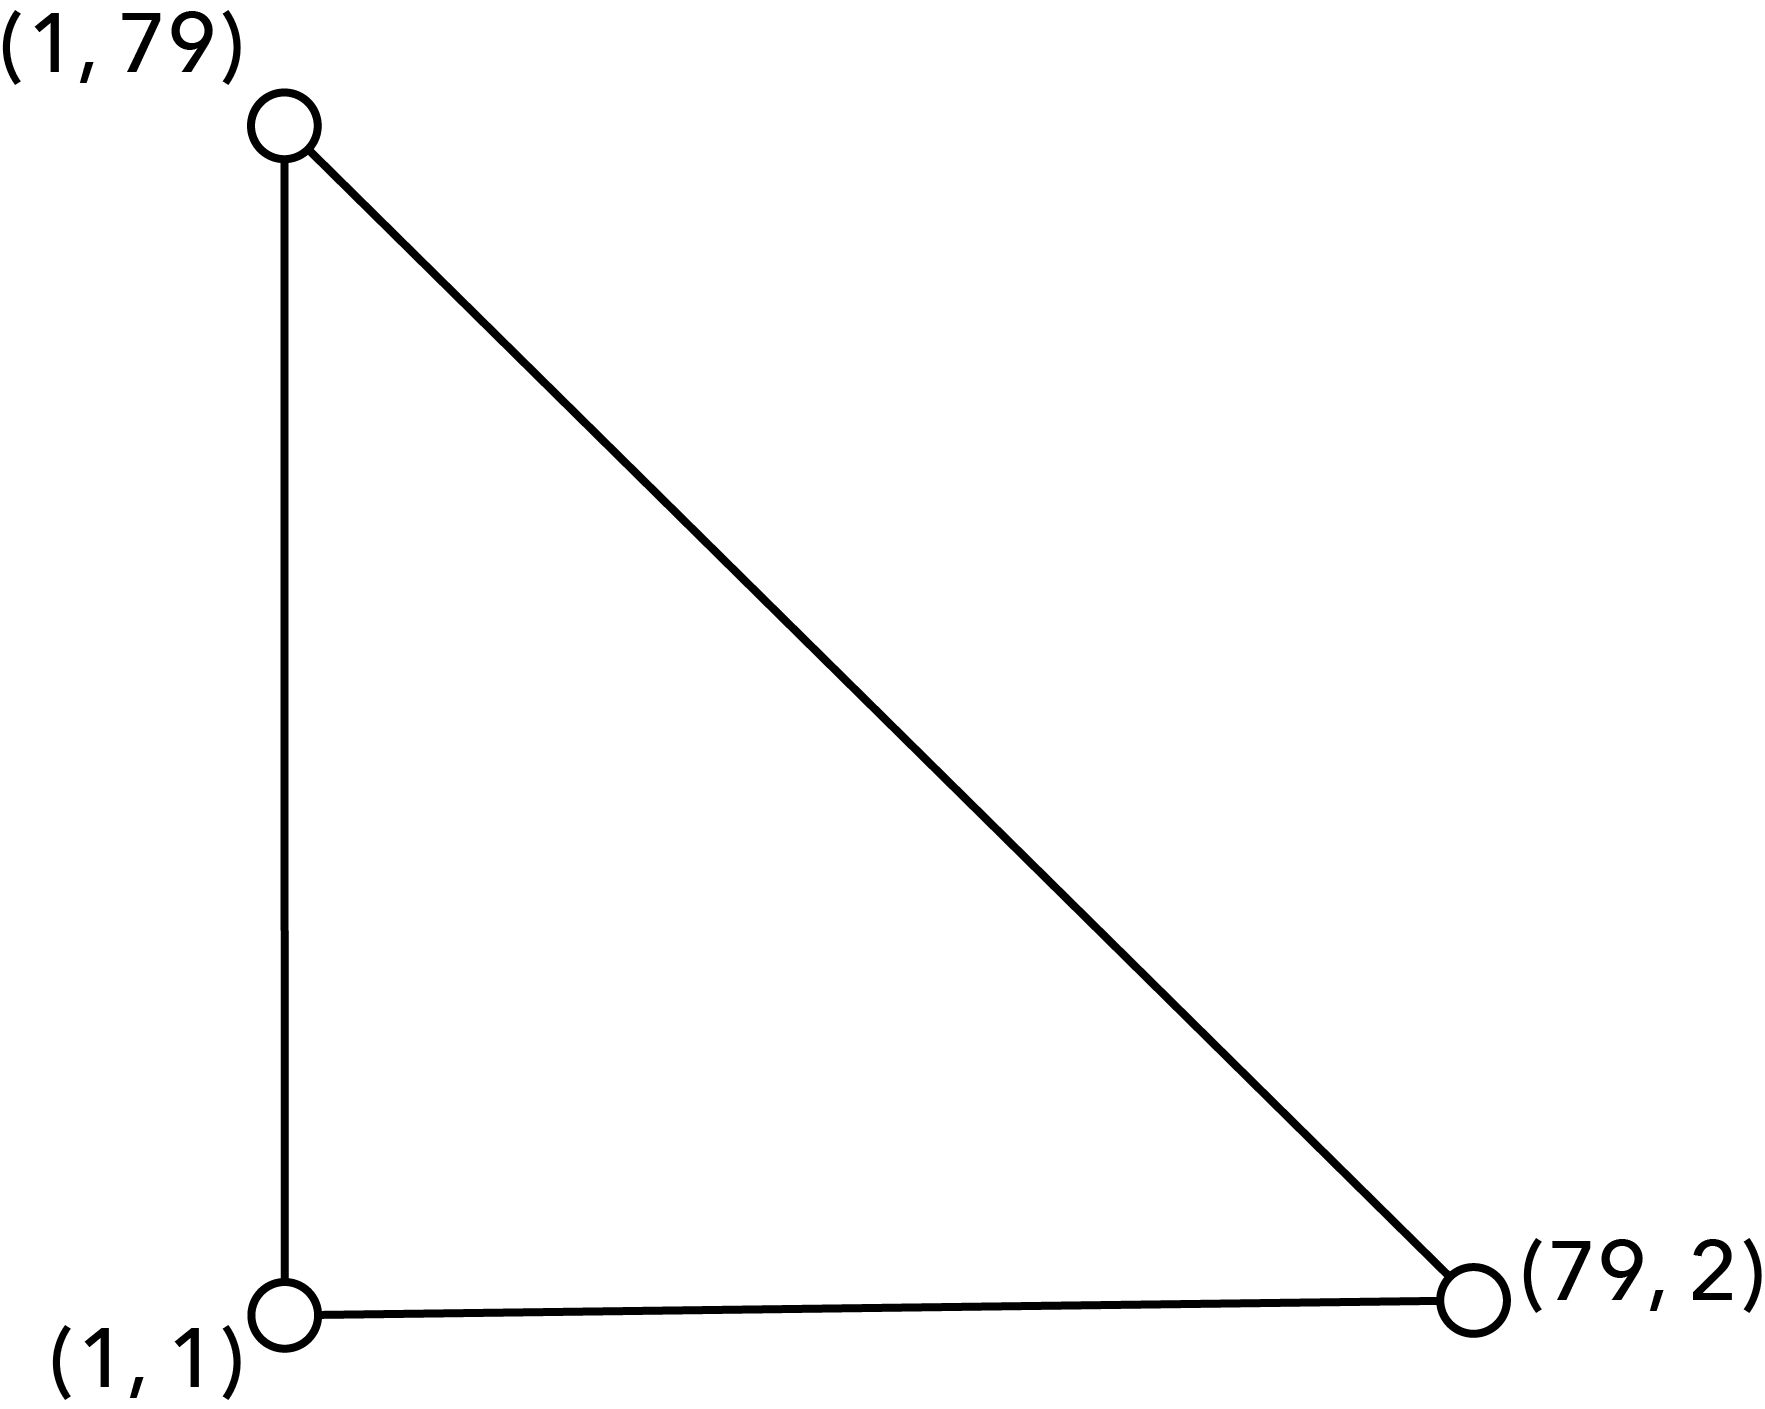
\includegraphics[width=0.35\linewidth]{../images/v-e-f/sol8.png}
    \end{figure}
    
    \vspace{18pt}
    
    큰 삼각형을 이렇게 만들어봅시다.
\end{frame}

\begin{frame}{\textbf{K}. 데이터 제작}
    삼각형 내부에
    \begin{itemize}
        \item $y = 78$인 점 1개
        \item $y = 77$인 점 2개
        \item $\ldots$
        \item $y = i$인 점 $(79-i)$개
    \end{itemize}
    를 넣을 수 있습니다.
    
    \vspace{18pt}
    
    총 $3 + \frac{78 \times 79}{2} = 3084$개의 점을 만들 수 있고, 이는 $3000$개의 점을 넣기에 충분합니다.
\end{frame}

\begin{frame}{\textbf{K}. 데이터 제작}
    $3N-6$개의 간선을 이용해 삼각형으로 쪼개는 방법은 아래 그림과 같이 하면 됩니다.
    
    \begin{figure}[h!]
        \centering
        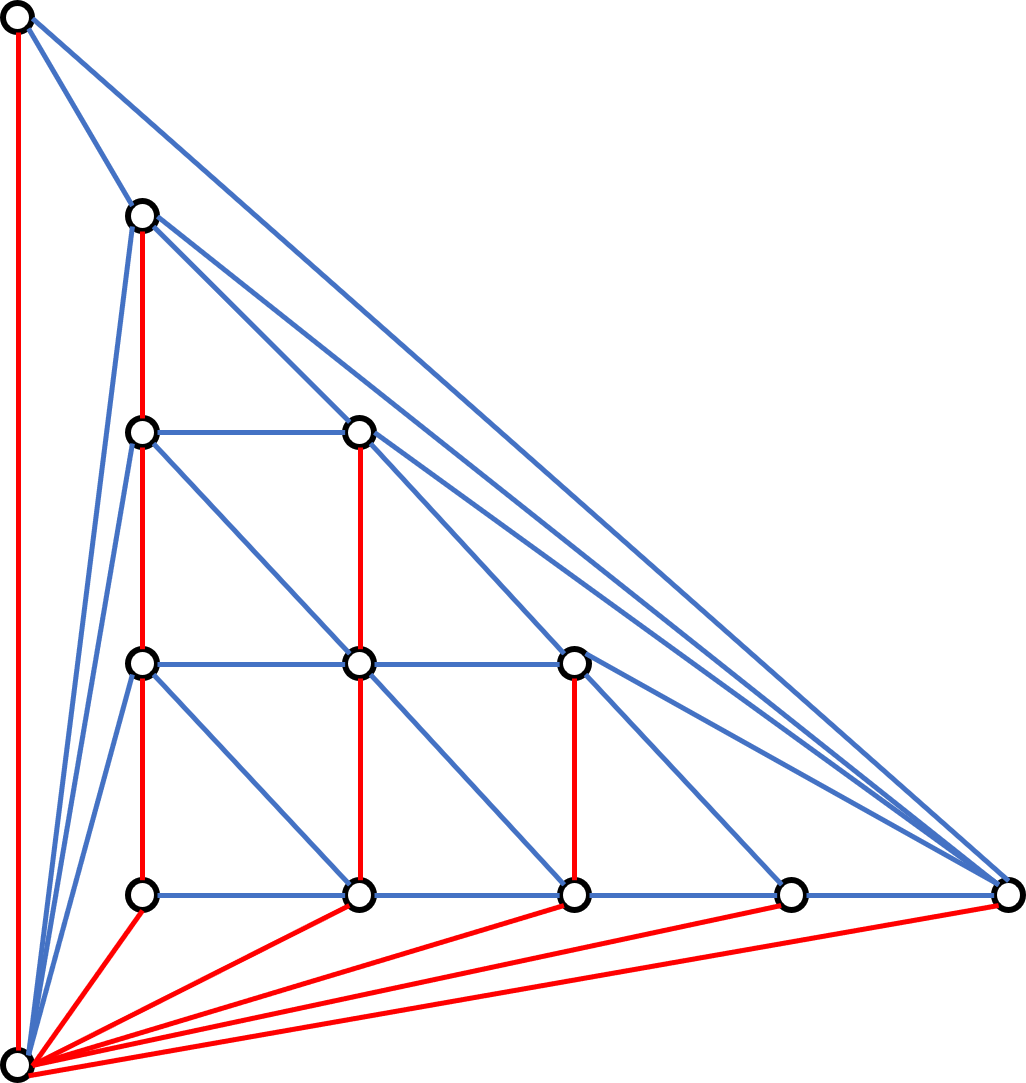
\includegraphics[width=0.30\linewidth]{../images/v-e-f/sol7.png}
    \end{figure}
    
    빨간 간선은 정점들이 연결 그래프를 이루기 위해서 꼭 필요한 간선이고\\
    파란색 간선은 $M$의 값에 따라 제거해도 되는 간선입니다.
\end{frame}

\begin{frame}{\textbf{K}. 데이터 제작}
    $M$값에 따라 파란색 간선을 적절히 추가/제거해서 원하는 그래프를 만들 수 있습니다.
    
    $C \neq 1$인 경우에는 남은 정점 $C-1$개를 큰 삼각형 영역 바깥쪽에 배치해주면 됩니다.
\end{frame}